\documentclass[a4paper,12pt]{article}

\usepackage{prettylatex}
\usepackage{titlepage}
\usepackage{boiboites}
\usepackage{pgfplots}

\top{Université de Technologie de Belfort-Montbéliard}{}
\title{Cours d'IN41}{Chapitre 3 -- Analyse des signaux apériodiques}
\author{}
\date{Semestre de printemps 2016}

\newboxedtheorem[boxcolor=orange, background={rgb:white,20;green,2;black,1}, titlebackground={rgb:white,15;green,5;black,3},
titleboxcolor = black]{defi}{Définition}{cmpDefi}

\begin{document}

\maketitlepage

\tableofcontents
\pagebreak

\section{Passage de la décomposition en séries de Fourier (DSF) à la transformée de Fourier (TF)}

Le passage d'un signal périodique à un signal apériodique peut se faire en considérant que la période $T$ devient de plus en plus grande pour tendre finalement vers $+\infty$.

\begin{defi}[Signal apériodique]
    Un signal apériodique $x(t)$ peut être défini à l'aide de son intégrale de Fourier
    \[ x(t) = \int_{-\infty}^{+\infty} X(if) e^{i2\pi ft} \mathrm{d}f \]
    \[ X(if) = \int_{-\infty}^{+\infty} x(t) e^{-i2\pi ft} \mathrm{d}t \]

    $X(if)$ est la transformée de Fourier directe de $x(t)$. $x(t)$ est la transformée de Fourier inverse de $X(if)$.
    \[ X(if) = \TF{x(t)} \]
    \[ x(t) = \mathrm{TF}^{-1} \{X(if)\} \]
\end{defi}

La courbe $X(if)$ en fonction de la fréquence f est le spectre du signal x. Si le signal $x(t)$ ne possède pas de symétries particulières, sa densité spectrale d'amplitude est une fonction complexe :
\[ x(t) \xrightarrow{\mathrm{TF}} X(if) = X_r(if) + iX_i(if) \]

La décomposition d'un signal $x(t)$ en ses composantes spectrales ($\TF{x(t)} = X(if)$) à l'aide de la transformée de Fourier porte le nom d'analyse spectrale ou analyse de Fourier.

Inversement, la synthèse d'un signal à l'aide de la transformée de Fourier inverse est la synthèse ou synthèse de Fourier.

\subsection{Propriétés}

\paragraph{Linéarité :}

\[
\begin{rcases}
    x(t) \xrightarrow{\mathrm{TF}} X(if) \\
    y(t) \xrightarrow{\mathrm{TF}} Y(if)
\end{rcases} \implies ax(t) + by(t) \xrightarrow{\mathrm{TF}} aX(if) + bY(if) \text{ avec } (a,b) \in \mathbb{C}^2\]

Donc la transformée de Fourier est une transformation linéaire.

\paragraph{Décalage temporel :}

\[ x(t) \xrightarrow{\mathrm{TF}} X(if) \]
\[ x(t + t_0) \xrightarrow{\mathrm{TF}} X(if) e^{i2\pi ft_0} \]

\subsubsection{Décalage fréquentiel}

\[ x(t) \xrightarrow{\mathrm{TF}} X(if) \]
\[ x(t) e^{i2\pi f_0t} \xrightarrow{\mathrm{TF}} X(i(f-f_p)) \]

\paragraph{Changement d'échelle :}

\[ \TF{ x(at)} = \dfrac{1}{||a||} X(i(\dfrac{f}{a})) \text{ avec } a \neq 0 \]

\paragraph{Parité :}

Si le signal $x$ est pair :
\[ X(if) = 2 \int_{0}^{+\infty} x(t) \cos(2\pi ft) \mathrm{d}t \]

Si le signal $x$ est impair :
\[ X(if) = -2i \int_{0}^{+\infty} x(t) \sin(2\pi ft) \mathrm{d}t \]

\paragraph{Spectre d'une impulsion rectangulaire $\mathrm{rect}_{\Delta t}(t)$ de largeur $\Delta t$ :}

\begin{figure}[!htbp]
	\centering
    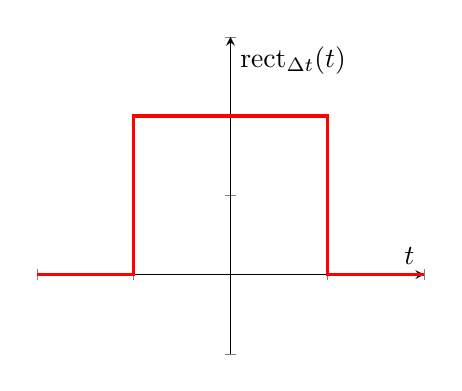
\begin{tikzpicture}
    	\begin{axis}[
            small, axis x line=middle, axis y line=center, xlabel=$t$, ylabel=$\mathrm{rect}_{\Delta t}(t)$, xmin=-4, xmax=4, ymin=-0.5, ymax=1.5,
            xticklabels={,,}, % to hide the numbers on the x axis
            yticklabels={,,} % to hide the numbers on the y axis
            ]
            \addplot+[very thick, red, mark=none, const plot] coordinates {(-4,0) (-2,1) (2,0) (4,0)};
    	\end{axis}
    \end{tikzpicture}
	\caption{Représentation d'une impulsion rectangulaire}
\end{figure}

\[ \mathrm{rect}_{\Delta t}(t) =
\begin{cases}
    A & \text{ si } |t| \leq \dfrac{\Delta t}{2} \\
    0 & \text{ sinon}
\end{cases} \]

Spectre de $\mathrm{rect}_{\Delta t}(t)$ :
\[ \mathrm{RECT}_{\Delta t}(if) = \TF{ \mathrm{rect}_{\Delta t}(t)} \]
\[ = \int_{-\infty}^{+\infty} \mathrm{rect}_{\Delta t}(t) e^{-i2\pi ft} \mathrm{d}t \]
\[ = \int_{-\Delta t / 2}^{\Delta t / 2} A e^{-i2\pi ft} \mathrm{d}t \]
\[ = A[\dfrac{e^{-i2\pi ft}}{-i2\pi f}]_{-\Delta t / 2}^{\Delta t / 2} \]
\[ = \dfrac{A}{\pi f} (\dfrac{e^{i\pi f\Delta t} - e^{-i\pi f\Delta t}}{2i}) \]
\[ = \dfrac{A\Delta t}{\pi f \Delta t} \sin(\pi f\Delta t) \]
\[ = \mathrm{sinc}(\pi f\Delta t) = A\Delta t \times \mathrm{sinc}(\pi f\Delta t) = \TF{ \mathrm{rect}_{\Delta t}(t)} \]

La densité spectrale d'amplitude d'nue impulsion rectangulaire centrée en t=0 est donnée par un sinus cardinal.

\paragraph{Spectre d'un sinus amorti}

\[ y(t) = \begin{cases}
    0 & \text{ si } t < 0 \\
    Ae^{-at} \sin(2\pi f_pt) \text{ si } t \geq 0
\end{cases} \]
\[ Y(if) = A\dfrac{2\pi f_p}{(s + i2\pi f)^2 + (2\pi f_p)^2} \in \mathbb{C} \]

\paragraph{Spectre de deux impulsions}

\begin{figure}[!htbp]
	\centering
    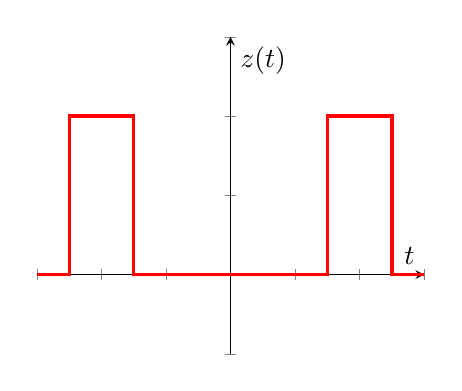
\begin{tikzpicture}
    	\begin{axis}[
            small, axis x line=middle, axis y line=center, xlabel=$t$, ylabel=$z(t)$, xmin=-6, xmax=6, ymin=-0.5, ymax=1.5,
            xticklabels={,,}, % to hide the numbers on the x axis
            yticklabels={,,} % to hide the numbers on the y axis
            ]
            \addplot+[very thick, red, mark=none, const plot] coordinates {(-6,0) (-5,1) (-3, 0) (3,1) (5,0) (6,0)};
    	\end{axis}
    \end{tikzpicture}
	\caption{Représentation de deux impulsions rectangulaires}
\end{figure}

\[ z(t) = \mathrm{rect}_{\Delta t}(t - \dfrac{t_0}{2}) + \mathrm{rect}_{\Delta t}(t + \dfrac{t_0}{2}) \]

Comme la transformée de Fourier est linéaire et $\TF{ x(t + t_0)} = X(if)e^{i2\pi ft_0}$, on a :
\[ Z(if) = 2A\Delta t \times \mathrm{sinc}(\underbrace{\pi f\Delta t)(e^{-i\pi ft_0} + e^{i\pi ft_0}}_{cos(\pi ft_0)}) \]

\paragraph{Spectre de l'exponentielle décroissante :}
\[ x(t) = \begin{cases}
    0 & \text{ si } t < 0 \\
    e^{-at} \text{ si } t \geq 0
\end{cases} \]
\[ X(if) = \dfrac{1}{a+i2\pi f} \]

\paragraph{Spectre de l'exponentielle décroissante symétrique :}
\[ x(t) = e^{-a|t|} \text{ avec } t \in \mathbb{R} \]
\[ X(if) = \dfrac{2a}{a^2+(2\pi f)^2} \]

\paragraph{Spectre du signal unité :}

\begin{figure}[!htbp]
	\centering
    \begin{tikzpicture}
    	\begin{axis}[
            small, axis x line=middle, axis y line=center, xlabel=$t$, ylabel=$z(t)$, xmin=-6, xmax=6, ymin=-0.5, ymax=1.5,
            xticklabels={,,}, % to hide the numbers on the x axis
            yticklabels={,,} % to hide the numbers on the y axis
            ]
            \addplot+[very thick, red, mark=none, const plot] coordinates {(-6,1) (6,1)};
    	\end{axis}
    \end{tikzpicture}
	\caption{Représentation de deux impulsions rectangulaires}
\end{figure}

Le signal $x(t) = 1, \forall t \in \mathbb{R}$ peut être décrit à partir de l'exponentielle décroissante :
\[ x(t) = 1 = \lim_{a \to 0} e^{-a|t|} \text{ avec } t \in \mathbb{R} \]
\[ \TF{ x(t)} = \int_{-\infty}^{+\infty} \lim_{a \to 0} e^{-a|t|} e^{-i2\pi ft} \mathrm{d}t \]
\[ X(if) = \lim_{a \to 0} \dfrac{2a}{a^2 + (2\pi f)^2} = \begin{cases}
    0 & \text{ si } f \neq 0 \\
    +\infty & \text{ si } f = 0
\end{cases} \]

On obtient une impulsion de Dirac :
\[ \TF{ x(t) = 1} = X(if) = \delta(f) \]

\paragraph{Spectre d'un phaseur}

Un phaseur de fréquence $f_0$ peut s'écrire :
\[ x(t) = e^{i2\pi f_0t} = \lim_{a \to 0} e^{-a|t|} e^{i2\pi f_0t} \]

En utilisant :
\[ \begin{cases}
    \TF{ e^{-a|t|} = \dfrac{2a}{a^2 + (2\pi f)^2}} \\
    x(t)e^{i2\pi ft} \xrightarrow{\mathrm{TF}} X(i(f-f_0))
\end{cases} \]

on a :
\[ X(if) = \lim_{a \to 0} \dfrac{2a}{a^2 + (2\pi(f-f_0))^2} \]
\[ = \begin{cases}
    +\infty & \text{ si } f = f_0 \\
    0 & \text{ si } f \neq f_0
\end{cases} \]

Donc la transformée de Fourier d'un phaseur de fréquence $f_0$ est une impulsion de Dirac située en $f=f_0$ :
\[ X(if) = \delta(f-f_0) \]

\paragraph{Spectre d'un signal sinusoïdal :}

Un signal sinusoïdal peut être vu comme la somme de deux phaseurs complexes conjugués.

\[ x(t) = \cos(2\pi f_0 t) = \dfrac{e^{i2\pi f_0t} + e^{-i2\pi f_0t}}{2} \]
\[ \implies X(if) = \TF{ \dfrac{1}{2} e^{i2\pi f_0t} + \dfrac{1}{2} e^{-i2\pi f_0t}} \]
\[ = \dfrac{1}{2} \TF{e^{i2\pi f_0t}} + \dfrac{1}{2} \TF{e^{i2\pi (-f_0)t}} \]
\[ = \dfrac{1}{2} \delta(f-f_0) + \dfrac{1}{2} \delta(f+f_0) \]

\end{document}
